\documentclass[bare_jrnl_transmag]{subfiles}
\begin{document}

\subsection{System Architecture}

The overall architecture for the algorithm can be broken into two parallel steps. On one side, the IMU data is read, and the pose is estimated using the Madgwick filter. The estimated pose and new acceleration from the IMU are fed into the Kalman Filter as the new states to determine a predicted new position. 

On the other side, the camera data is processed and filtered for features to determine changes in position, which are fed into the Kalman filter as the measurements.
git 
The Kalman filter fuses the two sensor inputs together to generate the new pose and position of the drone. 

Figure \ref{fig:vio-arch} shows the overall architecture of the algorithm. 

\begin{figure}
    [H]
    \centering
    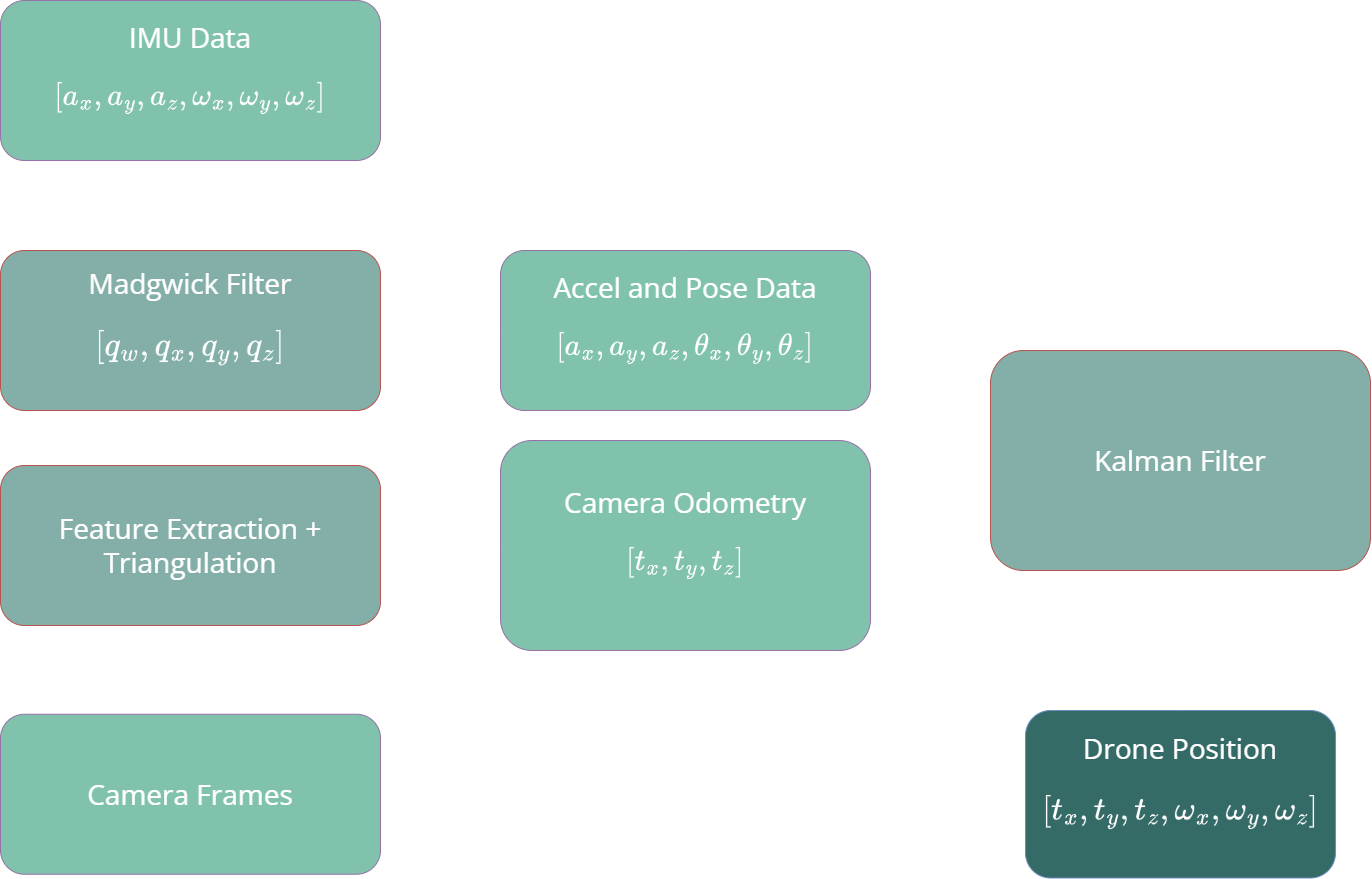
\includegraphics[width=0.8\linewidth]{figures/VIO-arch.png}
    \caption{VIO Algorithm architecture}
    \label{fig:vio-arch}
\end{figure}


\subsection{Assumptions}

For the system to function with the proposed algorithm, several assumptions were required. 
The first assumption is that the environment is unknown. The initial position is marked as the start point of the dataset but nothing else is known about the environment.

The second assumption made was that the stereo images were synced in time. If there was a small delay in capture, this could result in a skew in the position assumption.

TThe final assumption made was that the state of the drone cannot undergo a large change between time steps. This assumption is important because the prediction step of the Kalman filter uses previous states to calculate the new position. If the time step is too large, or if there was a very large change between time steps, the prediction would diverge very quickly at that point.  

\end{document}